\documentclass[twoside]{book}

% Packages required by doxygen
\usepackage{fixltx2e}
\usepackage{calc}
\usepackage{doxygen}
\usepackage[export]{adjustbox} % also loads graphicx
\usepackage{graphicx}
\usepackage[utf8]{inputenc}
\usepackage{makeidx}
\usepackage{multicol}
\usepackage{multirow}
\PassOptionsToPackage{warn}{textcomp}
\usepackage{textcomp}
\usepackage[nointegrals]{wasysym}
\usepackage[table]{xcolor}

% Font selection
\usepackage[T1]{fontenc}
\usepackage[scaled=.90]{helvet}
\usepackage{courier}
\usepackage{amssymb}
\usepackage{sectsty}
\renewcommand{\familydefault}{\sfdefault}
\allsectionsfont{%
  \fontseries{bc}\selectfont%
  \color{darkgray}%
}
\renewcommand{\DoxyLabelFont}{%
  \fontseries{bc}\selectfont%
  \color{darkgray}%
}
\newcommand{\+}{\discretionary{\mbox{\scriptsize$\hookleftarrow$}}{}{}}

% Page & text layout
\usepackage{geometry}
\geometry{%
  a4paper,%
  top=2.5cm,%
  bottom=2.5cm,%
  left=2.5cm,%
  right=2.5cm%
}
\tolerance=750
\hfuzz=15pt
\hbadness=750
\setlength{\emergencystretch}{15pt}
\setlength{\parindent}{0cm}
\setlength{\parskip}{3ex plus 2ex minus 2ex}
\makeatletter
\renewcommand{\paragraph}{%
  \@startsection{paragraph}{4}{0ex}{-1.0ex}{1.0ex}{%
    \normalfont\normalsize\bfseries\SS@parafont%
  }%
}
\renewcommand{\subparagraph}{%
  \@startsection{subparagraph}{5}{0ex}{-1.0ex}{1.0ex}{%
    \normalfont\normalsize\bfseries\SS@subparafont%
  }%
}
\makeatother

% Headers & footers
\usepackage{fancyhdr}
\pagestyle{fancyplain}
\fancyhead[LE]{\fancyplain{}{\bfseries\thepage}}
\fancyhead[CE]{\fancyplain{}{}}
\fancyhead[RE]{\fancyplain{}{\bfseries\leftmark}}
\fancyhead[LO]{\fancyplain{}{\bfseries\rightmark}}
\fancyhead[CO]{\fancyplain{}{}}
\fancyhead[RO]{\fancyplain{}{\bfseries\thepage}}
\fancyfoot[LE]{\fancyplain{}{}}
\fancyfoot[CE]{\fancyplain{}{}}
\fancyfoot[RE]{\fancyplain{}{\bfseries\scriptsize Generated by Doxygen }}
\fancyfoot[LO]{\fancyplain{}{\bfseries\scriptsize Generated by Doxygen }}
\fancyfoot[CO]{\fancyplain{}{}}
\fancyfoot[RO]{\fancyplain{}{}}
\renewcommand{\footrulewidth}{0.4pt}
\renewcommand{\chaptermark}[1]{%
  \markboth{#1}{}%
}
\renewcommand{\sectionmark}[1]{%
  \markright{\thesection\ #1}%
}

% Indices & bibliography
\usepackage{natbib}
\usepackage[titles]{tocloft}
\setcounter{tocdepth}{3}
\setcounter{secnumdepth}{5}
\makeindex

% Hyperlinks (required, but should be loaded last)
\usepackage{ifpdf}
\ifpdf
  \usepackage[pdftex,pagebackref=true]{hyperref}
\else
  \usepackage[ps2pdf,pagebackref=true]{hyperref}
\fi
\hypersetup{%
  colorlinks=true,%
  linkcolor=blue,%
  citecolor=blue,%
  unicode%
}

% Custom commands
\newcommand{\clearemptydoublepage}{%
  \newpage{\pagestyle{empty}\cleardoublepage}%
}

\usepackage{caption}
\captionsetup{labelsep=space,justification=centering,font={bf},singlelinecheck=off,skip=4pt,position=top}

%===== C O N T E N T S =====

\begin{document}

% Titlepage & ToC
\hypersetup{pageanchor=false,
             bookmarksnumbered=true,
             pdfencoding=unicode
            }
\pagenumbering{alph}
\begin{titlepage}
\vspace*{7cm}
\begin{center}%
{\Large Builder }\\
\vspace*{1cm}
{\large Generated by Doxygen 1.8.13}\\
\end{center}
\end{titlepage}
\clearemptydoublepage
\pagenumbering{roman}
\tableofcontents
\clearemptydoublepage
\pagenumbering{arabic}
\hypersetup{pageanchor=true}

%--- Begin generated contents ---
\chapter{Namespace Index}
\section{Packages}
Here are the packages with brief descriptions (if available)\+:\begin{DoxyCompactList}
\item\contentsline{section}{\hyperlink{namespace_decorator}{Decorator} }{\pageref{namespace_decorator}}{}
\end{DoxyCompactList}

\chapter{Hierarchical Index}
\section{Class Hierarchy}
This inheritance list is sorted roughly, but not completely, alphabetically\+:\begin{DoxyCompactList}
\item \contentsline{section}{Strategy.\+Dojazd}{\pageref{interface_strategy_1_1_dojazd}}{}
\begin{DoxyCompactList}
\item \contentsline{section}{Strategy.\+Rower}{\pageref{class_strategy_1_1_rower}}{}
\item \contentsline{section}{Strategy.\+Samochod}{\pageref{class_strategy_1_1_samochod}}{}
\end{DoxyCompactList}
\item \contentsline{section}{Strategy.\+Praca}{\pageref{interface_strategy_1_1_praca}}{}
\begin{DoxyCompactList}
\item \contentsline{section}{Strategy.\+Maluje\+Samochod}{\pageref{class_strategy_1_1_maluje_samochod}}{}
\item \contentsline{section}{Strategy.\+Montuje\+Silnik}{\pageref{class_strategy_1_1_montuje_silnik}}{}
\item \contentsline{section}{Strategy.\+Testuje\+Samochodow}{\pageref{class_strategy_1_1_testuje_samochodow}}{}
\end{DoxyCompactList}
\item \contentsline{section}{Strategy.\+Pracownik}{\pageref{class_strategy_1_1_pracownik}}{}
\item \contentsline{section}{Strategy.\+Spedzanie\+Wolnego\+Czasu}{\pageref{interface_strategy_1_1_spedzanie_wolnego_czasu}}{}
\begin{DoxyCompactList}
\item \contentsline{section}{Strategy.\+Gra\+Komputerowa}{\pageref{class_strategy_1_1_gra_komputerowa}}{}
\item \contentsline{section}{Strategy.\+Literatura\+Popularno\+Naukowa}{\pageref{class_strategy_1_1_literatura_popularno_naukowa}}{}
\item \contentsline{section}{Strategy.\+Silownia}{\pageref{class_strategy_1_1_silownia}}{}
\end{DoxyCompactList}
\item \contentsline{section}{Strategy.\+Strategy}{\pageref{class_strategy_1_1_strategy}}{}
\end{DoxyCompactList}

\chapter{Class Index}
\section{Class List}
Here are the classes, structs, unions and interfaces with brief descriptions\+:\begin{DoxyCompactList}
\item\contentsline{section}{\hyperlink{class_lazy_1_1_custom_lazy_class}{Lazy.\+Custom\+Lazy\+Class} \\*\hyperlink{class_lazy_1_1_custom_lazy_class}{Custom\+Lazy\+Class} posiada zmienna \+\_\+\+Value inicjalizowaną tuż przed uzyciem }{\pageref{class_lazy_1_1_custom_lazy_class}}{}
\item\contentsline{section}{\hyperlink{class_lazy_1_1_lazy}{Lazy.\+Lazy} \\*Klasa zawierająca funkcje Main }{\pageref{class_lazy_1_1_lazy}}{}
\item\contentsline{section}{\hyperlink{class_lazy_1_1_lazy_class}{Lazy.\+Lazy\+Class} \\*\hyperlink{class_lazy_1_1_lazy_class}{Lazy\+Class} posiada zmienna Value }{\pageref{class_lazy_1_1_lazy_class}}{}
\end{DoxyCompactList}

\chapter{Namespace Documentation}
\hypertarget{namespace_builder}{}\section{Builder Namespace Reference}
\label{namespace_builder}\index{Builder@{Builder}}
\subsection*{Classes}
\begin{DoxyCompactItemize}
\item 
class \hyperlink{class_builder_1_1_program}{Program}
\end{DoxyCompactItemize}

\chapter{Class Documentation}
\hypertarget{class_builder_1_1_program_1_1_builder}{}\section{Builder.\+Program.\+Builder Class Reference}
\label{class_builder_1_1_program_1_1_builder}\index{Builder.\+Program.\+Builder@{Builder.\+Program.\+Builder}}


Glowny interface  


Inheritance diagram for Builder.\+Program.\+Builder\+:\begin{figure}[H]
\begin{center}
\leavevmode
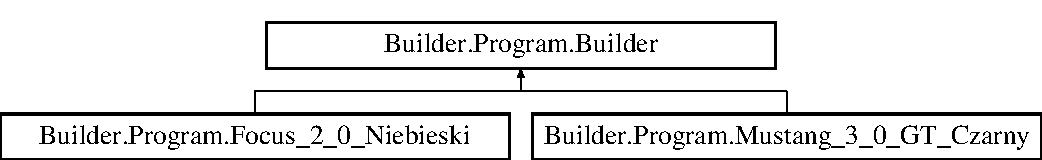
\includegraphics[height=2.000000cm]{class_builder_1_1_program_1_1_builder}
\end{center}
\end{figure}
\subsection*{Public Member Functions}
\begin{DoxyCompactItemize}
\item 
\mbox{\Hypertarget{class_builder_1_1_program_1_1_builder_a965509ae45286ca38694a876774a9c09}\label{class_builder_1_1_program_1_1_builder_a965509ae45286ca38694a876774a9c09}} 
void {\bfseries new\+Samochod} ()
\item 
\mbox{\Hypertarget{class_builder_1_1_program_1_1_builder_a5ab500d83d0f5a82839b58548a16f457}\label{class_builder_1_1_program_1_1_builder_a5ab500d83d0f5a82839b58548a16f457}} 
\hyperlink{class_builder_1_1_program_1_1_samochod}{Samochod} {\bfseries get\+Samochod} ()
\item 
\mbox{\Hypertarget{class_builder_1_1_program_1_1_builder_a8193cb0bd469b75298af2a0b1bf654da}\label{class_builder_1_1_program_1_1_builder_a8193cb0bd469b75298af2a0b1bf654da}} 
abstract void {\bfseries build\+Silnik} ()
\item 
\mbox{\Hypertarget{class_builder_1_1_program_1_1_builder_a40ad407267df66a335fc765f9ee62608}\label{class_builder_1_1_program_1_1_builder_a40ad407267df66a335fc765f9ee62608}} 
abstract void {\bfseries build\+Kategoria} ()
\item 
\mbox{\Hypertarget{class_builder_1_1_program_1_1_builder_a4116b74aa9e501068d7341c837631870}\label{class_builder_1_1_program_1_1_builder_a4116b74aa9e501068d7341c837631870}} 
abstract void {\bfseries build\+Kolor} ()
\item 
\mbox{\Hypertarget{class_builder_1_1_program_1_1_builder_a9aad5c49ff78651d5e66139cf31d1c43}\label{class_builder_1_1_program_1_1_builder_a9aad5c49ff78651d5e66139cf31d1c43}} 
abstract void {\bfseries build\+Nazwa} ()
\end{DoxyCompactItemize}
\subsection*{Protected Attributes}
\begin{DoxyCompactItemize}
\item 
\mbox{\Hypertarget{class_builder_1_1_program_1_1_builder_a8bedc36c849a81f778fef38d4d8677ee}\label{class_builder_1_1_program_1_1_builder_a8bedc36c849a81f778fef38d4d8677ee}} 
\hyperlink{class_builder_1_1_program_1_1_samochod}{Samochod} {\bfseries samochod}
\end{DoxyCompactItemize}


\subsection{Detailed Description}
Glowny interface 



The documentation for this class was generated from the following file\+:\begin{DoxyCompactItemize}
\item 
Program.\+cs\end{DoxyCompactItemize}

\hypertarget{class_builder_1_1_program_1_1_director}{}\section{Builder.\+Program.\+Director Class Reference}
\label{class_builder_1_1_program_1_1_director}\index{Builder.\+Program.\+Director@{Builder.\+Program.\+Director}}


Klasa zlecająca builderom zbudowanie obiektu  


\subsection*{Public Member Functions}
\begin{DoxyCompactItemize}
\item 
\mbox{\Hypertarget{class_builder_1_1_program_1_1_director_a5fb8365b0b81938e4364d01f8d61b696}\label{class_builder_1_1_program_1_1_director_a5fb8365b0b81938e4364d01f8d61b696}} 
void {\bfseries set\+Builder} (\hyperlink{class_builder_1_1_program_1_1_builder}{Builder} builder)
\item 
\mbox{\Hypertarget{class_builder_1_1_program_1_1_director_ab055442d8b92dda823881f4d5d062c39}\label{class_builder_1_1_program_1_1_director_ab055442d8b92dda823881f4d5d062c39}} 
\hyperlink{class_builder_1_1_program_1_1_samochod}{Samochod} {\bfseries get\+Samochod} ()
\item 
\mbox{\Hypertarget{class_builder_1_1_program_1_1_director_a5426a035af6a76cc18b2dd15a450df55}\label{class_builder_1_1_program_1_1_director_a5426a035af6a76cc18b2dd15a450df55}} 
void {\bfseries Produkuj} ()
\end{DoxyCompactItemize}


\subsection{Detailed Description}
Klasa zlecająca builderom zbudowanie obiektu 



The documentation for this class was generated from the following file\+:\begin{DoxyCompactItemize}
\item 
Program.\+cs\end{DoxyCompactItemize}

\hypertarget{class_builder_1_1_program_1_1_focus__2__0___niebieski}{}\section{Builder.\+Program.\+Focus\+\_\+2\+\_\+0\+\_\+\+Niebieski Class Reference}
\label{class_builder_1_1_program_1_1_focus__2__0___niebieski}\index{Builder.\+Program.\+Focus\+\_\+2\+\_\+0\+\_\+\+Niebieski@{Builder.\+Program.\+Focus\+\_\+2\+\_\+0\+\_\+\+Niebieski}}


\hyperlink{class_builder_1_1_program_1_1_focus__2__0___niebieski}{Focus\+\_\+2\+\_\+0\+\_\+\+Niebieski} implementuje inteface \hyperlink{class_builder_1_1_program_1_1_builder}{Builder} dzieki czemu precyzujemy wartości obiektu  


Inheritance diagram for Builder.\+Program.\+Focus\+\_\+2\+\_\+0\+\_\+\+Niebieski\+:\begin{figure}[H]
\begin{center}
\leavevmode
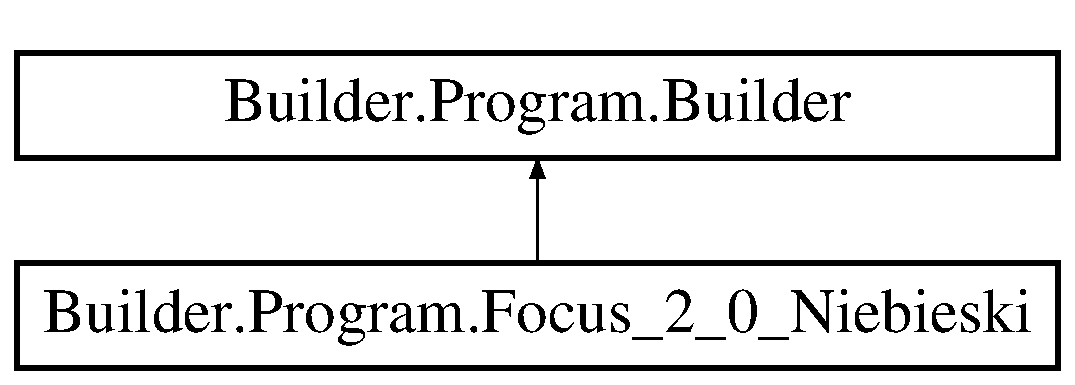
\includegraphics[height=2.000000cm]{class_builder_1_1_program_1_1_focus__2__0___niebieski}
\end{center}
\end{figure}
\subsection*{Public Member Functions}
\begin{DoxyCompactItemize}
\item 
\mbox{\Hypertarget{class_builder_1_1_program_1_1_focus__2__0___niebieski_aa65fca28aadf7ca55a89a6d07bc067b2}\label{class_builder_1_1_program_1_1_focus__2__0___niebieski_aa65fca28aadf7ca55a89a6d07bc067b2}} 
override void {\bfseries build\+Silnik} ()
\item 
\mbox{\Hypertarget{class_builder_1_1_program_1_1_focus__2__0___niebieski_af9bf66e45cd2b1d649dd1bb7c969729a}\label{class_builder_1_1_program_1_1_focus__2__0___niebieski_af9bf66e45cd2b1d649dd1bb7c969729a}} 
override void {\bfseries build\+Kategoria} ()
\item 
\mbox{\Hypertarget{class_builder_1_1_program_1_1_focus__2__0___niebieski_a23eaa690b38376d674d5d6c419403257}\label{class_builder_1_1_program_1_1_focus__2__0___niebieski_a23eaa690b38376d674d5d6c419403257}} 
override void {\bfseries build\+Kolor} ()
\item 
\mbox{\Hypertarget{class_builder_1_1_program_1_1_focus__2__0___niebieski_a53d0f8e360205daf15b50a3d84b48b4b}\label{class_builder_1_1_program_1_1_focus__2__0___niebieski_a53d0f8e360205daf15b50a3d84b48b4b}} 
override void {\bfseries build\+Nazwa} ()
\end{DoxyCompactItemize}
\subsection*{Additional Inherited Members}


\subsection{Detailed Description}
\hyperlink{class_builder_1_1_program_1_1_focus__2__0___niebieski}{Focus\+\_\+2\+\_\+0\+\_\+\+Niebieski} implementuje inteface \hyperlink{class_builder_1_1_program_1_1_builder}{Builder} dzieki czemu precyzujemy wartości obiektu 



The documentation for this class was generated from the following file\+:\begin{DoxyCompactItemize}
\item 
Program.\+cs\end{DoxyCompactItemize}

\hypertarget{class_builder_1_1_program_1_1_mustang__3__0___g_t___czarny}{}\section{Builder.\+Program.\+Mustang\+\_\+3\+\_\+0\+\_\+\+G\+T\+\_\+\+Czarny Class Reference}
\label{class_builder_1_1_program_1_1_mustang__3__0___g_t___czarny}\index{Builder.\+Program.\+Mustang\+\_\+3\+\_\+0\+\_\+\+G\+T\+\_\+\+Czarny@{Builder.\+Program.\+Mustang\+\_\+3\+\_\+0\+\_\+\+G\+T\+\_\+\+Czarny}}


\hyperlink{class_builder_1_1_program_1_1_mustang__3__0___g_t___czarny}{Mustang\+\_\+3\+\_\+0\+\_\+\+G\+T\+\_\+\+Czarny} implementuje inteface \hyperlink{class_builder_1_1_program_1_1_builder}{Builder} dzieki czemu precyzujemy wartości obiektu  


Inheritance diagram for Builder.\+Program.\+Mustang\+\_\+3\+\_\+0\+\_\+\+G\+T\+\_\+\+Czarny\+:\begin{figure}[H]
\begin{center}
\leavevmode
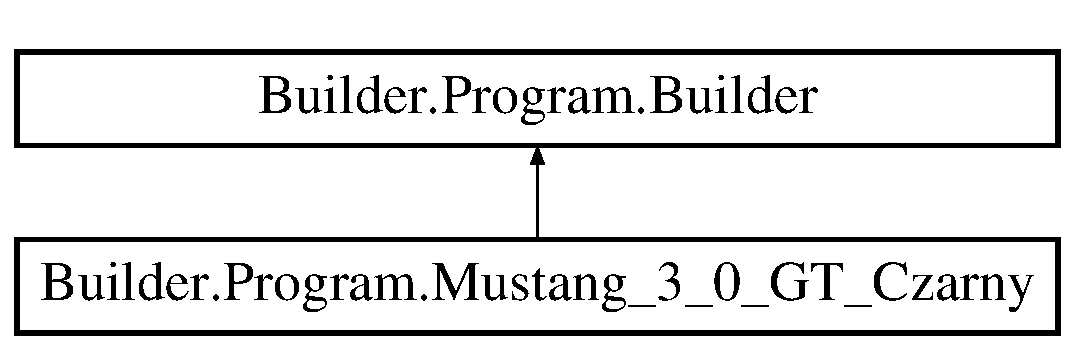
\includegraphics[height=2.000000cm]{class_builder_1_1_program_1_1_mustang__3__0___g_t___czarny}
\end{center}
\end{figure}
\subsection*{Public Member Functions}
\begin{DoxyCompactItemize}
\item 
\mbox{\Hypertarget{class_builder_1_1_program_1_1_mustang__3__0___g_t___czarny_a1d0fb9488ef4802206af0c2378115d7a}\label{class_builder_1_1_program_1_1_mustang__3__0___g_t___czarny_a1d0fb9488ef4802206af0c2378115d7a}} 
override void {\bfseries build\+Silnik} ()
\item 
\mbox{\Hypertarget{class_builder_1_1_program_1_1_mustang__3__0___g_t___czarny_adc30373d97de4d016604b9b93a9c55c1}\label{class_builder_1_1_program_1_1_mustang__3__0___g_t___czarny_adc30373d97de4d016604b9b93a9c55c1}} 
override void {\bfseries build\+Kategoria} ()
\item 
\mbox{\Hypertarget{class_builder_1_1_program_1_1_mustang__3__0___g_t___czarny_a1c82fa76d55453780b905baa74ad06d6}\label{class_builder_1_1_program_1_1_mustang__3__0___g_t___czarny_a1c82fa76d55453780b905baa74ad06d6}} 
override void {\bfseries build\+Kolor} ()
\item 
\mbox{\Hypertarget{class_builder_1_1_program_1_1_mustang__3__0___g_t___czarny_aae607f4545c14fd451690bb7c6f3309f}\label{class_builder_1_1_program_1_1_mustang__3__0___g_t___czarny_aae607f4545c14fd451690bb7c6f3309f}} 
override void {\bfseries build\+Nazwa} ()
\end{DoxyCompactItemize}
\subsection*{Additional Inherited Members}


\subsection{Detailed Description}
\hyperlink{class_builder_1_1_program_1_1_mustang__3__0___g_t___czarny}{Mustang\+\_\+3\+\_\+0\+\_\+\+G\+T\+\_\+\+Czarny} implementuje inteface \hyperlink{class_builder_1_1_program_1_1_builder}{Builder} dzieki czemu precyzujemy wartości obiektu 



The documentation for this class was generated from the following file\+:\begin{DoxyCompactItemize}
\item 
Program.\+cs\end{DoxyCompactItemize}

\hypertarget{class_builder_1_1_program}{}\section{Builder.\+Program Class Reference}
\label{class_builder_1_1_program}\index{Builder.\+Program@{Builder.\+Program}}
\subsection*{Classes}
\begin{DoxyCompactItemize}
\item 
class \hyperlink{class_builder_1_1_program_1_1_builder}{Builder}
\begin{DoxyCompactList}\small\item\em Glowny interface \end{DoxyCompactList}\item 
class \hyperlink{class_builder_1_1_program_1_1_director}{Director}
\begin{DoxyCompactList}\small\item\em Klasa zlecająca builderom zbudowanie obiektu \end{DoxyCompactList}\item 
class \hyperlink{class_builder_1_1_program_1_1_focus__2__0___niebieski}{Focus\+\_\+2\+\_\+0\+\_\+\+Niebieski}
\begin{DoxyCompactList}\small\item\em \hyperlink{class_builder_1_1_program_1_1_focus__2__0___niebieski}{Focus\+\_\+2\+\_\+0\+\_\+\+Niebieski} implementuje inteface \hyperlink{class_builder_1_1_program_1_1_builder}{Builder} dzieki czemu precyzujemy wartości obiektu \end{DoxyCompactList}\item 
class \hyperlink{class_builder_1_1_program_1_1_mustang__3__0___g_t___czarny}{Mustang\+\_\+3\+\_\+0\+\_\+\+G\+T\+\_\+\+Czarny}
\begin{DoxyCompactList}\small\item\em \hyperlink{class_builder_1_1_program_1_1_mustang__3__0___g_t___czarny}{Mustang\+\_\+3\+\_\+0\+\_\+\+G\+T\+\_\+\+Czarny} implementuje inteface \hyperlink{class_builder_1_1_program_1_1_builder}{Builder} dzieki czemu precyzujemy wartości obiektu \end{DoxyCompactList}\item 
class \hyperlink{class_builder_1_1_program_1_1_samochod}{Samochod}
\begin{DoxyCompactList}\small\item\em Klasa samochod posiada metody z których korzysta builder \end{DoxyCompactList}\end{DoxyCompactItemize}
\subsection*{Static Public Member Functions}
\begin{DoxyCompactItemize}
\item 
static void \hyperlink{class_builder_1_1_program_a414b7e29e16f01d915ac02dffa280ebc}{Main} (string\mbox{[}$\,$\mbox{]} args)
\begin{DoxyCompactList}\small\item\em Funkcja Main wywoluje kolejno funkcje oraz wyświetla wyniki \end{DoxyCompactList}\end{DoxyCompactItemize}


\subsection{Member Function Documentation}
\mbox{\Hypertarget{class_builder_1_1_program_a414b7e29e16f01d915ac02dffa280ebc}\label{class_builder_1_1_program_a414b7e29e16f01d915ac02dffa280ebc}} 
\index{Builder\+::\+Program@{Builder\+::\+Program}!Main@{Main}}
\index{Main@{Main}!Builder\+::\+Program@{Builder\+::\+Program}}
\subsubsection{\texorpdfstring{Main()}{Main()}}
{\footnotesize\ttfamily static void Builder.\+Program.\+Main (\begin{DoxyParamCaption}\item[{string \mbox{[}$\,$\mbox{]}}]{args }\end{DoxyParamCaption})\hspace{0.3cm}{\ttfamily [static]}}



Funkcja Main wywoluje kolejno funkcje oraz wyświetla wyniki 


\begin{DoxyParams}{Parameters}
{\em args} & Standardowy zapis funkcji Main z parametrem args\\
\hline
\end{DoxyParams}


The documentation for this class was generated from the following file\+:\begin{DoxyCompactItemize}
\item 
Program.\+cs\end{DoxyCompactItemize}

\hypertarget{class_builder_1_1_program_1_1_samochod}{}\section{Builder.\+Program.\+Samochod Class Reference}
\label{class_builder_1_1_program_1_1_samochod}\index{Builder.\+Program.\+Samochod@{Builder.\+Program.\+Samochod}}


Klasa samochod posiada metody z których korzysta builder  


\subsection*{Public Member Functions}
\begin{DoxyCompactItemize}
\item 
\mbox{\Hypertarget{class_builder_1_1_program_1_1_samochod_af4d2eb9e389cfebc9170e7c079bc944d}\label{class_builder_1_1_program_1_1_samochod_af4d2eb9e389cfebc9170e7c079bc944d}} 
void {\bfseries set\+Silnik} (String silnik)
\item 
\mbox{\Hypertarget{class_builder_1_1_program_1_1_samochod_a284af3a9af1625ea7096fe9201772726}\label{class_builder_1_1_program_1_1_samochod_a284af3a9af1625ea7096fe9201772726}} 
void {\bfseries set\+Karoseria} (String karoseria)
\item 
\mbox{\Hypertarget{class_builder_1_1_program_1_1_samochod_a37ea3ffe0420269c297b6629c98cad4d}\label{class_builder_1_1_program_1_1_samochod_a37ea3ffe0420269c297b6629c98cad4d}} 
void {\bfseries set\+Kolor} (String kolor)
\item 
\mbox{\Hypertarget{class_builder_1_1_program_1_1_samochod_ae51c9e19c0d6dd0121e0d2c376ce50a5}\label{class_builder_1_1_program_1_1_samochod_ae51c9e19c0d6dd0121e0d2c376ce50a5}} 
void {\bfseries set\+Nazwa} (String nazwa)
\item 
\mbox{\Hypertarget{class_builder_1_1_program_1_1_samochod_a672fa98295ff4dd32320f42feda2420c}\label{class_builder_1_1_program_1_1_samochod_a672fa98295ff4dd32320f42feda2420c}} 
void {\bfseries show} ()
\end{DoxyCompactItemize}
\subsection*{Properties}
\begin{DoxyCompactItemize}
\item 
\mbox{\Hypertarget{class_builder_1_1_program_1_1_samochod_ac36ea3564bfbea3fad2ed821b62bd757}\label{class_builder_1_1_program_1_1_samochod_ac36ea3564bfbea3fad2ed821b62bd757}} 
String {\bfseries silnik}\hspace{0.3cm}{\ttfamily  \mbox{[}get, set\mbox{]}}
\item 
\mbox{\Hypertarget{class_builder_1_1_program_1_1_samochod_ae11c5804edf3abb6b78ad4b62ca0d4ac}\label{class_builder_1_1_program_1_1_samochod_ae11c5804edf3abb6b78ad4b62ca0d4ac}} 
String {\bfseries karoseria}\hspace{0.3cm}{\ttfamily  \mbox{[}get, set\mbox{]}}
\item 
\mbox{\Hypertarget{class_builder_1_1_program_1_1_samochod_a1c9be9a1d5768a8fea406444d64163e2}\label{class_builder_1_1_program_1_1_samochod_a1c9be9a1d5768a8fea406444d64163e2}} 
String {\bfseries kolor}\hspace{0.3cm}{\ttfamily  \mbox{[}get, set\mbox{]}}
\item 
\mbox{\Hypertarget{class_builder_1_1_program_1_1_samochod_aab4d403164b723dbd367a08dfa689fde}\label{class_builder_1_1_program_1_1_samochod_aab4d403164b723dbd367a08dfa689fde}} 
String {\bfseries nazwa}\hspace{0.3cm}{\ttfamily  \mbox{[}get, set\mbox{]}}
\end{DoxyCompactItemize}


\subsection{Detailed Description}
Klasa samochod posiada metody z których korzysta builder 



The documentation for this class was generated from the following file\+:\begin{DoxyCompactItemize}
\item 
Program.\+cs\end{DoxyCompactItemize}

%--- End generated contents ---

% Index
\backmatter
\newpage
\phantomsection
\clearemptydoublepage
\addcontentsline{toc}{chapter}{Index}
\printindex

\end{document}
